% !TEX root = relatorio.tex
%
% Capítulo 5 — Implementação
%
\chapter{Implementação} \label{cap:implementacao}

O Capítulo~\ref{cap:desenvolvimento} desenhou o Play4Change em silhueta: dois clientes que nunca falam diretamente com quem gera, guarda ou protege o que consomem; um perímetro que filtra e autentica antes de qualquer pedido chegar à lógica de negócio; um núcleo que decide; e quatro capacidades externas de que esse núcleo depende sem nunca as referenciar diretamente. Este capítulo preenche essa silhueta, peça a peça: começamos pelo servidor e pela porta de entrada (Secção~\ref{sec:backend}), seguimos o conteúdo desde a submissão pelo Administrador até ao tópico pronto para um Learner se inscrever (Secção~\ref{sec:conteudo-desafio}), acompanhamos o Learner no seu percurso diário (Secção~\ref{sec:percurso-learner}), e fechamos com a segurança que atravessa tudo isto (Secção~\ref{sec:seguranca-impl}). Os \textit{prompts} completos enviados ao modelo em cada uma destas fases estão reproduzidos, sem alterações, no Apêndice~\ref{ap:prompts}.

% =====================================================================
\section{Fundações: Servidor, Pipeline e Autenticação} \label{sec:backend}
% =====================================================================

Os dois clientes do Play4Change (o painel web do Administrador e a aplicação móvel do Learner) precisam de um ponto de entrada único para falar com o núcleo do sistema, capaz de servir da mesma forma um browser e um telemóvel. A forma mais direta de o fazer é uma API RESTful: sem estado entre pedidos, organizada por recursos, e igualmente natural para os dois lados. É essa API que o servidor expõe.

O servidor é escrito em Kotlin sobre Spring Boot~3 (JVM~21), com as regras de negócio isoladas de Spring, JPA ou de qualquer fornecedor externo concreto: a mesma indireção do Capítulo~\ref{cap:desenvolvimento}, agora ao nível do código.

É esta última camada que dá corpo às quatro capacidades externas do Capítulo~\ref{cap:desenvolvimento}. Persistir e indexar cai sobre PostgreSQL, via JPA; gerar conteúdo pedagógico cai sobre um módulo dedicado que fala com o Mistral através do LangChain4j, isolado nos seus próprios módulos Gradle (\texttt{ai-agent:api} e \texttt{ai-agent:langchain}): trocar de fornecedor de IA implica escrever um novo adaptador, não tocar numa linha de lógica de negócio; extrair conteúdo cai sobre Playwright e Unstructured.io, detalhados na Secção~\ref{sec:conteudo-desafio}; e notificar o utilizador cai sobre Resend para email e \textit{Server-Sent Events} para progresso em tempo real.

Como o domínio do sistema cresce ao longo do projeto, o esquema da base de dados precisa de evoluir com ele sem arriscar o que já lá está. Essa evolução é gerida exclusivamente por Flyway: cada alteração é um ficheiro SQL versionado e registado em git, aplicado pela mesma ordem em qualquer ambiente (33 até à data).

\subsection{Pipeline de Processamento de Pedidos} \label{sec:pipeline}

\begin{figure}[H]
    \centering
    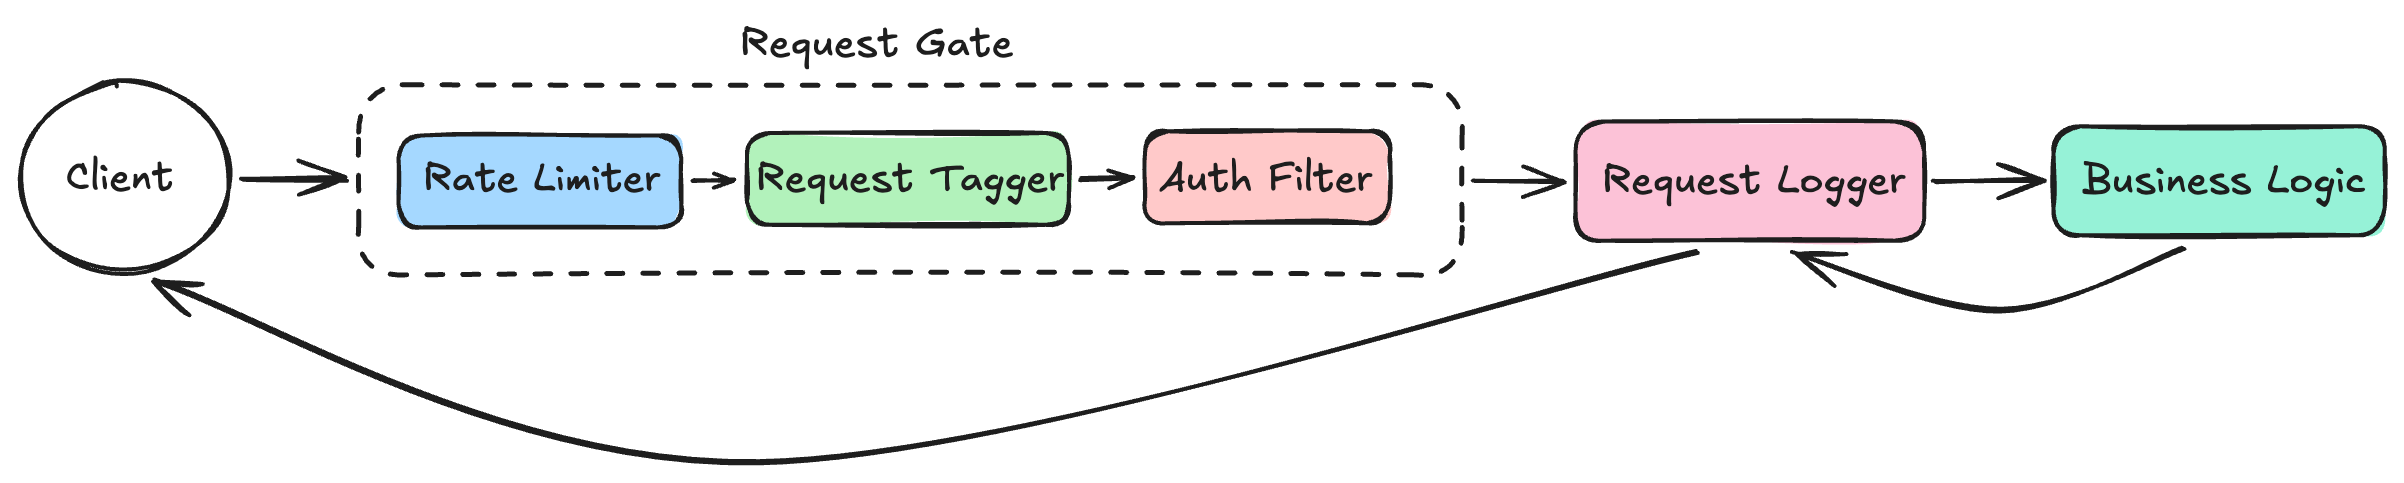
\includegraphics[width=\textwidth]{./figures/Request-Diagram.png}
    \caption{Percurso de um pedido HTTP até à lógica de negócio}
    \label{fig:request-pipeline}
\end{figure}

A Figura~\ref{fig:request-pipeline} resume o percurso de um pedido até chegar a um \textit{controller}. Antes disso, todo o pedido atravessa um \textit{Request Gate} de três filtros, e a ordem lá dentro não é arbitrária: um sistema que gera conteúdo por IA a pedido é um alvo natural de abuso, pelo que a primeira pergunta que qualquer pedido enfrenta não é ``quem és'', mas ``quantos pedidos já fizeste''. O \textit{Rate Limiter} corre por isso antes de qualquer autenticação (o que trava tentativas de força bruta mesmo contra quem ainda não tem sessão) e responde \texttt{429 Too Many Requests}, o código pensado precisamente para isto (ao contrário de um \texttt{403}, que assinalaria uma identidade já conhecida mas sem permissão). Mais à frente na mesma cadeia, o \textit{Auth Filter} responde \texttt{401 Unauthorized} quando o token falha: o código reservado para identidade ausente ou inválida, não para uma identidade válida sem privilégios suficientes (esse caso é \texttt{403}, adiante). Um pedido travado por qualquer um dos dois não chega ao \textit{Request Logger}: fica sem o identificador de correlação do \textit{Request Tagger} e sem entrada nos registos. Só o que atravessa o Gate por completo é identificado, registado e chega à lógica de negócio. \label{sec:ratelimiting}

O \textit{Request Logger} regista o pedido duas vezes, não uma: à entrada, antes da lógica de negócio, e à saída, depois dela: é esse par que permite medir, nos registos, quanto tempo cada pedido demorou do princípio ao fim.

O limite exato depende do \textit{endpoint} (Tabela~\ref{tab:rate-limits-endpoint}): mais apertado onde a frequência esperada é baixa e o risco alto (pedido de código de acesso, para prevenir \textit{email bombing}, e criação ou regeneração de um tópico, porque cada pedido despoleta uma chamada à API da Mistral, pelo que o limite protege também contra custo descontrolado); mais permissivo na submissão de tarefas (30 pedidos/10~min), invocada com muito mais frequência em uso legítimo, mas ainda assim suficiente para travar \textit{brute-forcing} de respostas.

\begin{longtable}{lll}
\caption{Limites de \textit{rate limiting} por endpoint (janela de reabastecimento de 10 minutos em todos os casos)} \label{tab:rate-limits-endpoint} \\
\hline
\textbf{Endpoint} & \textbf{Limite} & \textbf{Janela} \\
\hline
\endfirsthead
\multicolumn{3}{l}{\small\textit{Tabela~\ref{tab:rate-limits-endpoint} (continuação)}} \\
\hline
\textbf{Endpoint} & \textbf{Limite} & \textbf{Janela} \\
\hline
\endhead
\hline
\multicolumn{3}{r}{\small\textit{continua na página seguinte}} \\
\endfoot
\hline
\endlastfoot
\texttt{POST /auth/magic-link}                              & 5 pedidos  & 10 min \\
\texttt{POST /auth/magic-link/verify}                        & 10 pedidos & 10 min \\
\texttt{POST /auth/verify}                                   & 10 pedidos & 10 min \\
\texttt{POST /auth/oauth}                                    & 10 pedidos & 10 min \\
\texttt{POST /auth/refresh}                                  & 20 pedidos & 10 min \\
\texttt{POST /auth/logout}                                   & 10 pedidos & 10 min \\
\texttt{POST /auth/recovery-email/verify}                    & 10 pedidos & 10 min \\
\texttt{POST /admin/topics}                                  & 3 pedidos  & 10 min \\
\texttt{POST /admin/topics/pdf}                               & 2 pedidos  & 10 min \\
\texttt{POST /admin/topics/\{id\}/regenerate}                 & 2 pedidos  & 10 min \\
\texttt{POST /tasks/\{id\}/submit}                            & 30 pedidos & 10 min \\
\texttt{POST /struggle/\{id\}/tasks/\{id\}/submit}            & 30 pedidos & 10 min \\
\texttt{POST /explanation/\{id\}/message}                     & 10 pedidos & 10 min \\
\end{longtable}

Um pedido em particular não se resolve dentro desta cadeia: quando um Administrador submete um documento ou URL para gerar os desafios correspondentes por IA demora demasiado para o deixar à espera de uma resposta HTTP. Em vez de bloquear, o servidor confirma a submissão de imediato (\texttt{201 Created}) e passa o resto do trabalho para um executor dedicado, que progride por cinco estados:
\begin{center}
\texttt{INGESTION} $\rightarrow$ \texttt{ANALYSIS} $\rightarrow$ \texttt{GENERATION} $\rightarrow$ \texttt{INDEXING} $\rightarrow$ \texttt{ACTIVE}
\end{center}
(qualquer fase pode transitar para \texttt{FAILED}, e dois \textit{schedulers} Spring vigiam o pipeline: um marca como falhados os tópicos presos demasiado tempo em geração, outro expira os que já passaram do prazo). O \texttt{201 Created} encerra ali o pedido original: o acompanhamento do progresso não faz parte dele. Para o ver sem recarregar a página, o cliente abre, à parte, uma ligação de \textit{Server-Sent Events} a \texttt{GET /admin/topics/\{id\}/progress}, recebendo eventos de mudança de fase até à conclusão ou falha da geração. Esta máquina de estados é a espinha dorsal de tudo o que se segue na Secção~\ref{sec:conteudo-desafio}: cada uma das suas fases corresponde a um mecanismo concreto detalhado adiante.

\subsection{Autenticação sem Password} \label{sec:autenticacao}

Autenticar um pedido resume-se sempre à mesma mecânica: o utilizador prova a sua identidade uma vez, o servidor emite um token que a representa, e é esse token (não a prova original) que o Auth Filter valida a cada pedido seguinte (Secção~\ref{sec:pipeline}). O que muda de sistema para sistema é só essa primeira prova, a que acontece uma vez para depois nunca mais ser preciso repetir. A forma mais comum de a fazer, uma \textit{password}, é mal ajustada a este produto em particular: é vulnerável a reutilização entre serviços, força bruta e \textit{phishing}, frequentemente esquecida, e Bonneau et al.~\cite{bonneau2012} avaliam 35 esquemas alternativos sem encontrar um vencedor universal: os mais resistentes a ataques (tokens físicos, biometria) tendem a sacrificar exatamente a usabilidade em que as \textit{passwords} se destacam. Para um desafio breve e diário, dirigido também a um perfil de menor afinidade tecnológica (Secção~\ref{sec:usab-qualitativa}), a escolha caiu sobre um código de utilização única enviado por email, que o utilizador introduz para se autenticar. Isto elimina a fricção de memorização e o conceito de password esquecida, ao custo de a segurança e a recuperação da conta passarem a depender inteiramente do email do Learner, risco que o sistema mitiga com um email de recuperação alternativo como segunda via de acesso.

\begin{figure}[H]
    \centering
    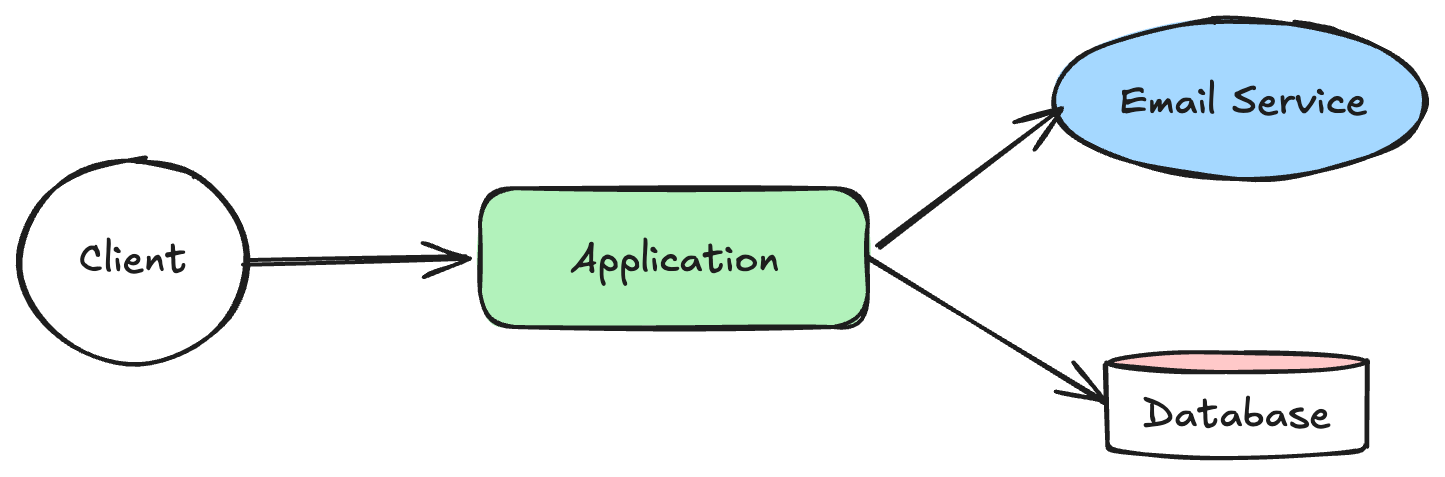
\includegraphics[width=0.75\textwidth]{./figures/Auth-Relation.png}
    \caption{Relação entre a aplicação e os serviços externos no pedido de código}
    \label{fig:auth-relation}
\end{figure}

A Figura~\ref{fig:auth-relation} mostra a relação por detrás deste pedido: a aplicação nunca fala com o email do utilizador nem com a base de dados por si só: pede a um serviço de email externo (Resend) que envie o código, e guarda na base de dados apenas o \textit{hash} SHA-256 desse código, nunca o valor em claro. Três decisões deliberadas fecham as frestas óbvias deste tipo de fluxo: o pedido do código responde sempre \texttt{202 Accepted} independentemente de o email existir, para não permitir a um atacante descobrir que contas existem; o consumo do código é uma operação atómica, para que dois pedidos em simultâneo não consigam ambos ter sucesso; e as três formas de falha (código inválido, expirado, ou já usado) são indistinguíveis para o cliente, para não dar pistas a quem tenta adivinhar. \label{sec:auth-flow}

Autenticado com sucesso, o Learner recebe um par de tokens, e cada um viaja e é guardado de forma diferente. O \textit{access token} JWT, de vida curta (15~min), vai no \textit{header} \texttt{Authorization: Bearer} de cada pedido seguinte e nunca é guardado no servidor: a própria assinatura chega para o validar (Secção~\ref{sec:pipeline}). O \textit{refresh token}, de vida mais longa (7~dias), vai apenas no corpo do pedido a \texttt{POST /auth/refresh} e é guardado no servidor unicamente como \textit{hash}, nunca em claro. Do lado do cliente, cada plataforma usa o seu próprio armazenamento seguro: \textit{Keychain} no iOS, \textit{EncryptedSharedPreferences} no Android, e um \textit{cookie} \texttt{SameSite=Strict} no painel web.

\begin{figure}[H]
    \centering
    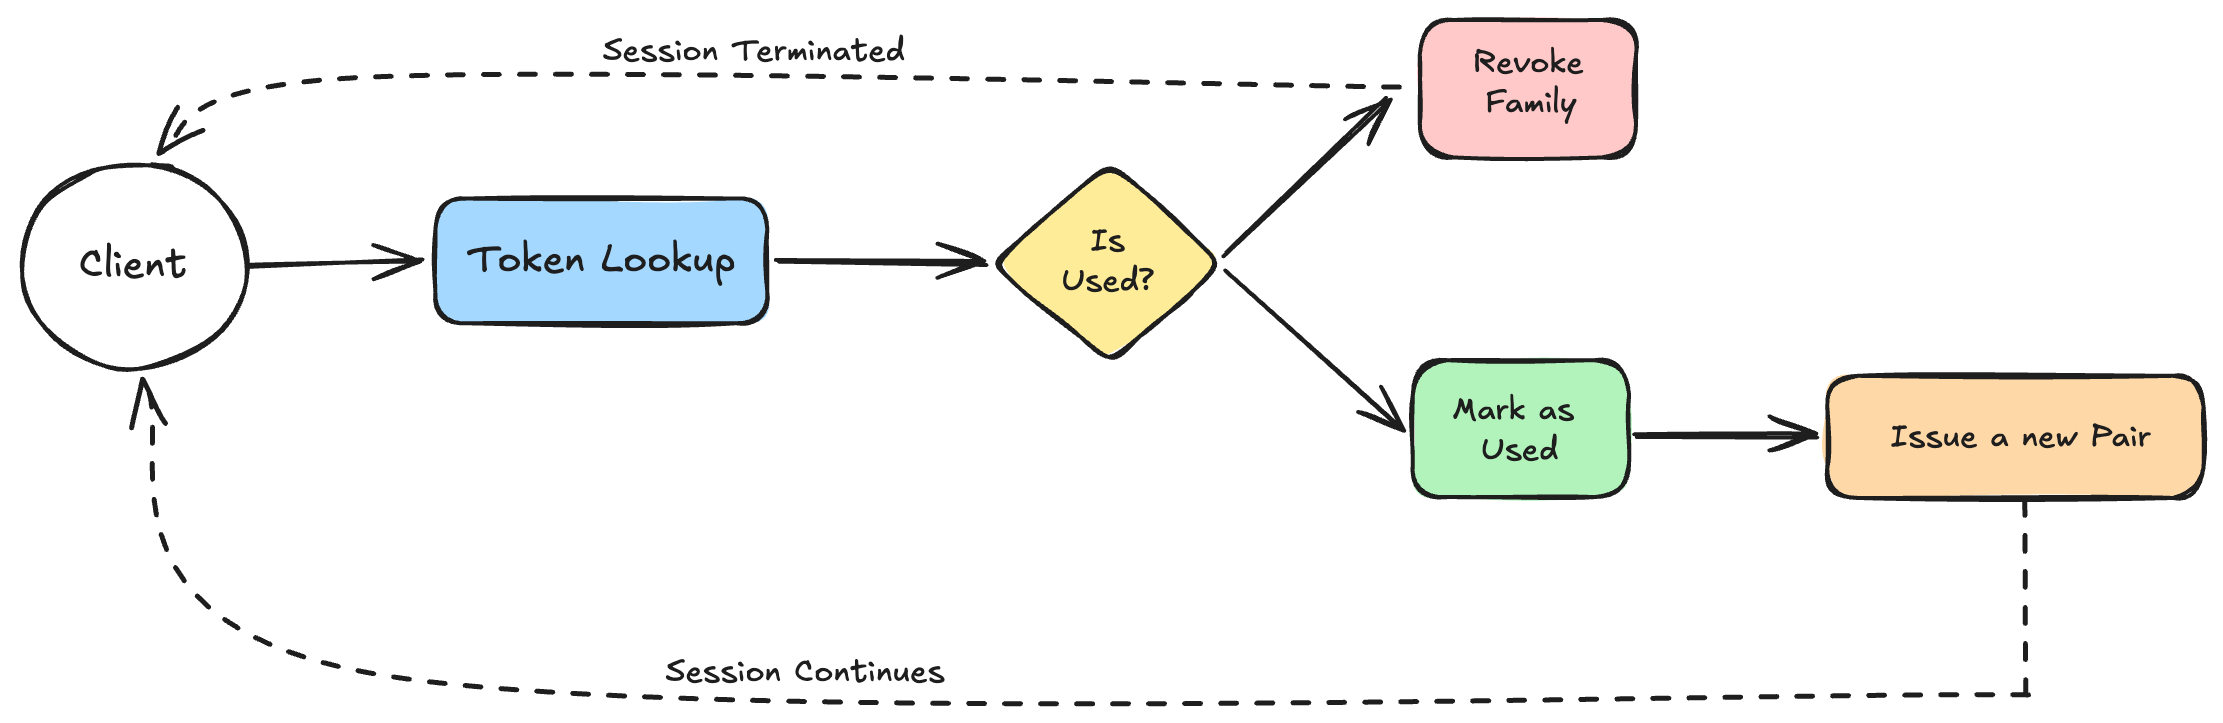
\includegraphics[width=\textwidth]{./figures/TokenReuse.png}
    \caption{Rotação do refresh token e deteção de reutilização}
    \label{fig:token-reuse}
\end{figure}

É o \textit{refresh token} que precisa de mais cuidado, precisamente por viver mais tempo: segue rotação com deteção de reutilização (Figura~\ref{fig:token-reuse}). A cada renovação, o token apresentado é procurado pelo seu \textit{hash} e marcado como usado antes de um novo par ser emitido, sempre associado à mesma família (\texttt{familyId}). Se esse mesmo token (já marcado como usado) for reapresentado, o sistema interpreta isso como sinal de roubo: revoga toda a família de uma vez, e o Learner tem de voltar a autenticar-se do zero. \label{sec:token-lifecycle} O acesso às rotas de administração exige o papel correspondente, validado a cada pedido contra o mesmo JWT; esse papel fica fixado na criação da conta (por omissão Learner) e só é elevado a Admin por edição manual direta na base de dados, nunca pela API pública nem por qualquer mecanismo de semente automatizado. \label{sec:authz}

% =====================================================================
\section{Do Conteúdo ao Desafio} \label{sec:conteudo-desafio}
% =====================================================================

Com o núcleo e a porta de entrada no lugar, faltam as duas metades que tornam o Play4Change mais do que um CRUD: como o conteúdo é criado, do lado do Administrador (Secção~\ref{cap:ingestao}), e como é consumido, do lado do Learner (Secção~\ref{sec:percurso-learner}).

\subsection{Criação do Conteúdo} \label{cap:ingestao}

Um Administrador começa sempre com pouco: um documento PDF ou o URL de uma página. O que tem de sair no fim não é um desafio isolado, é um \textbf{tópico} completo (com os seus módulos e desafios já gerados) pronto para um Learner se inscrever e, a partir daí, passar a receber um desafio novo desse tópico a cada dia. É esse caminho que a Figura~\ref{fig:topic-creation} resume e o resto desta subsecção percorre, zona a zona.

\begin{figure}[H]
    \centering
    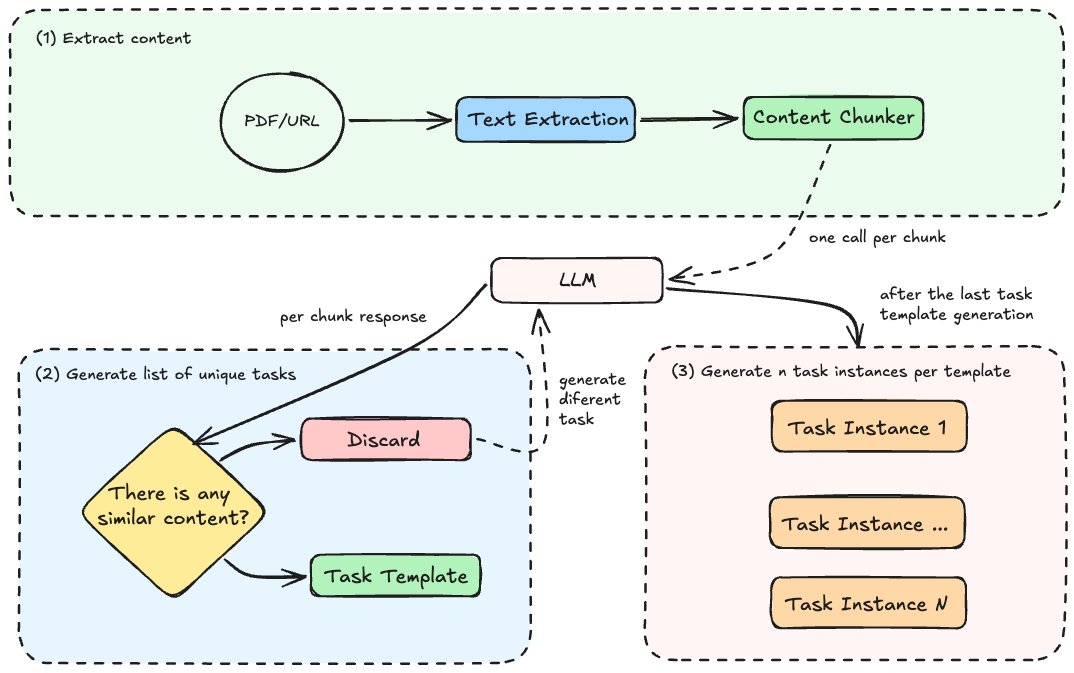
\includegraphics[width=\textwidth]{./figures/Topic-creation.png}
    \caption{Do conteúdo extraído ao desafio guardado: uma chamada por bloco, deduplicação antes de persistir, reposição dirigida quando falta quantidade}
    \label{fig:topic-creation}
\end{figure}

\subsubsection*{Antes da Zona (1): do Documento a Texto Simples}

Um PDF e uma página web exigem tecnologia genuinamente diferente para se tornarem texto, por isso a extração vive atrás de um único contrato, com duas implementações consoante a fonte:

\begin{itemize}
    \item \textbf{PDF}: a \textbf{Unstructured API}~\cite{unstructured2023}, escolhida pela necessidade de OCR (\textit{Optical Character Recognition}) em documentos digitalizados;
    \item \textbf{URL}: um microserviço \textbf{Playwright}~\cite{playwright2023}, necessário porque muitas páginas educativas são \textit{Single Page Applications} que só mostram conteúdo depois de executar JavaScript; uma chamada HTTP simples veria uma página vazia.
\end{itemize}

Um URL traz, porém, um risco que um PDF não traz: é o próprio servidor que vai buscá-lo, e nada impede, à partida, que aponte para um endereço interno da rede em vez de uma página pública. Antes de qualquer pedido de rede, o \texttt{UrlSsrfValidator} fecha essa porta: esquema \texttt{https} obrigatório, \textit{host} válido e, por resolução DNS, rejeição de endereços \textit{loopback}, de rede privada ou \textit{link-local}. \label{sec:url} \label{sec:pdf} \label{sec:limites-ingestao}

\subsubsection*{Zona (1) $\to$ Caixa ``LLM'': Uma Chamada por Bloco}

Com o texto já extraído, resta um último obstáculo antes de chegar ao modelo de IA: um documento inteiro raramente cabe num único \textit{prompt}, e mesmo que coubesse, seria caro processá-lo de uma vez. O \texttt{ContentChunker} particiona-o em blocos de 32\,000 caracteres com sobreposição de 2\,000, preferindo cortar em limites de parágrafo para não partir uma ideia a meio: é por isso que a seta só chega a ``LLM'' depois de extração e \textit{chunking}, um bloco de cada vez, nunca o documento inteiro. A caixa está rotulada de forma deliberadamente genérica: seja qual for o fornecedor por trás, a resposta a cada chamada é sempre um conjunto de tarefas candidatas para esse bloco, nunca uma tarefa isolada. Na versão atual, esse fornecedor é o \textbf{Mistral AI} (\texttt{mistral-small-latest}, via LangChain4j), escolhido por quatro razões: \label{sec:ia-prompting}

\begin{itemize}
    \item os \textit{prompts} são multilingues por natureza, e o modelo responde bem em várias línguas sem ajuste adicional;
    \item gerar uma questão de escolha múltipla não exige a capacidade de raciocínio de um modelo maior, pelo que um modelo mais pequeno chega, a um custo por chamada menor;
    \item o sistema depende de \textit{output} JSON estruturado e fiável, que o modelo cumpre de forma consistente;
    \item a arquitetura já garante que trocar de modelo, se um dia for preciso, não é uma reescrita (Secção~\ref{sec:arquitetura}).
\end{itemize}

Quantas tarefas cada chamada pede também não é fixo: o total definido pelo Administrador é repartido pelos blocos em proporção ao comprimento de cada um (\texttt{TaskCountAllocator}), não pedido na íntegra a cada bloco: um documento com dez secções e um pedido de cem tarefas produz cem no total, mais nas secções com mais conteúdo, menos nas mais curtas, e nunca próximo de mil com todas a mirar o mesmo alvo. Quando o total não é divisível de forma exata, o resto vai para os blocos cuja quota arredondada perdeu mais (método do maior resto), garantindo que a soma final corresponde sempre ao pedido.

Quando a chave de API não está definida, um adaptador \textit{no-op} responde \texttt{503} em vez de falhar em silêncio.

Nas duas primeiras finalidades do módulo de IA (gerar tarefas e sintetizar ramos de remediação), o que entra nesta caixa nunca é texto livre escrito por um utilizador: o \textit{user prompt} é sempre construído a partir de dados estruturados do próprio domínio (título do tópico, nível de audiência, padrão de erro), o que é, nesses dois casos, a primeira e mais eficaz defesa do sistema contra \textit{prompt injection} (Secção~\ref{sec:seguranca-impl}): não há \textit{input} a injetar onde não há \textit{input} nenhum. Já a terceira finalidade, a condução de sessões de explicação, recebe efetivamente o texto que o Learner escreve na conversa (Secção~\ref{sec:explicacao-ia}); nesse caso a defesa não é a ausência de \textit{input}, mas o isolamento desse \textit{input} na sua própria mensagem de origem não confiada, como descrito na Secção~\ref{sec:seguranca-impl}.

\subsubsection*{Zona (2): O Losango e o Retorno a ``LLM''}

Chamar o modelo tem um custo que cresce com o número de utilizadores e de tópicos, por isso cada candidata que sai dele passa primeiro por um filtro de semelhança, não é logo guardada. O seu texto é convertido numa espécie de impressão digital numérica (um vetor que resume o \textit{significado} da frase, não as palavras exatas), e essa impressão digital é comparada, uma a uma, com as de todas as tarefas já existentes no mesmo módulo. Se a semelhança for demasiado alta, a candidata é descartada como duplicado semântico, sem sequer chegar a ser persistida; caso contrário, torna-se um \texttt{TaskTemplate} definitivo. É esta inversão (usar recuperação vectorial para decidir se vale a pena gerar, em vez de para enriquecer o que se gera) que é a decisão de implementação mais original do sistema: quanto mais a base de conhecimento cresce, menos o custo de gerar cresce com ela. \label{cap:rag} \label{sec:armazenamento}

A pergunta óbvia que o losango levanta é o que acontece às descartadas: ficam simplesmente perdidas, reduzindo silenciosamente o número final de tarefas? Não: é essa a seta de retorno a ``LLM''. Se, no fim de um bloco, o número de tarefas aceites ficar abaixo do pedido, o sistema volta a chamar o modelo uma única vez, mas de forma dirigida, não às cegas: pede exatamente a diferença (se de dez pedidas nove forem aceites, pede uma, não as dez outra vez) e envia ao modelo, explicitamente, os títulos das tarefas já aceites nesse bloco e nos anteriores do mesmo tópico, para que a nova tentativa tenha uma hipótese real de ser diferente em vez de arriscar repetir o que já foi descartado. Como qualquer chamada de rede a um serviço externo, esta também pode falhar ou demorar; e, como é a chamada mais cara e mais lenta do sistema, está protegida por um \textit{timeout} de 60~segundos por bloco. Nesta fase a geração corre em segundo plano, do lado do Administrador, pelo que a falha de uma chamada não bloqueia ninguém; o que acontece ao bloco (e ao tópico) quando isso falha é explicado no fecho desta subsecção, na Zona (3).

\subsubsection*{Zona (3): As Caixas Laranja, Depois do Último \textit{Template}}

Gerar uma tarefa uma vez não chega: se todos os Learners inscritos no mesmo módulo vissem exatamente a mesma pergunta com as mesmas opções erradas, comparar respostas seria trivial. Por isso cada desafio existe em dois níveis:

\begin{itemize}
    \item \texttt{TaskTemplate}: a definição canónica gerada pelo LLM;
    \item até cinco \texttt{TaskInstance} por \textit{template}: variantes com distratores diferentes, que partilham a mesma resposta correta mas nunca as mesmas opções erradas.
\end{itemize}

Estas instâncias só são geradas depois de todos os blocos do documento terem terminado a sua fase de geração e os respetivos \textit{templates} estarem todos persistidos. Uma falha no primeiro bloco aborta a geração inteira; falhas em blocos seguintes são toleradas, preservando o que já foi persistido.

Nenhuma questão chega ao Learner sem passar por um conjunto de verificações simples que garantem que faz sentido. Antes de ser guardada, cada candidata é comparada em significado com as já existentes no mesmo módulo, para não repetir uma pergunta com outras palavras; o formato é validado: número certo de opções, resposta correta identificada de forma consistente; e confirma-se que está na língua e no nível de dificuldade pedidos. O texto que o modelo devolve é sempre limpo antes de persistir, para que não haja espaço para conteúdo indevido se infiltrar. E se o modelo falhar ou devolver algo incompleto, o sistema tenta corrigir automaticamente antes de desistir: nunca fica uma questão a meio guardada como se estivesse completa. É este conjunto de verificações, aplicado a cada questão individualmente, que garante a qualidade do conteúdo gerado, não uma auditoria posterior.

\subsection{Consumo do Conteúdo} \label{sec:percurso-learner}

O tópico já existe; falta o Learner inscrever-se nele, receber os seus desafios diários, tentar resolvê-los, e o sistema reagir ao resultado. Esta subsecção segue esse percurso do princípio ao fim, em três momentos: o pedido do desafio do dia, o que acontece quando a resposta falha, e o que acontece quando nem a remediação chega. Os três encadeiam-se num único ciclo.

\subsubsection{Atribuição Diária} \label{cap:desafios} \label{sec:atribuicao}

Em vez de o sistema calcular e enviar um desafio a cada utilizador todos os dias (o que exigiria um processo em segundo plano a correr para toda a base de Learners), é o Learner que pede o seu ao abrir a aplicação. A Figura~\ref{fig:daily-challenge} resume esse pedido e o que acontece depois de responder.

\begin{figure}[H]
    \centering
    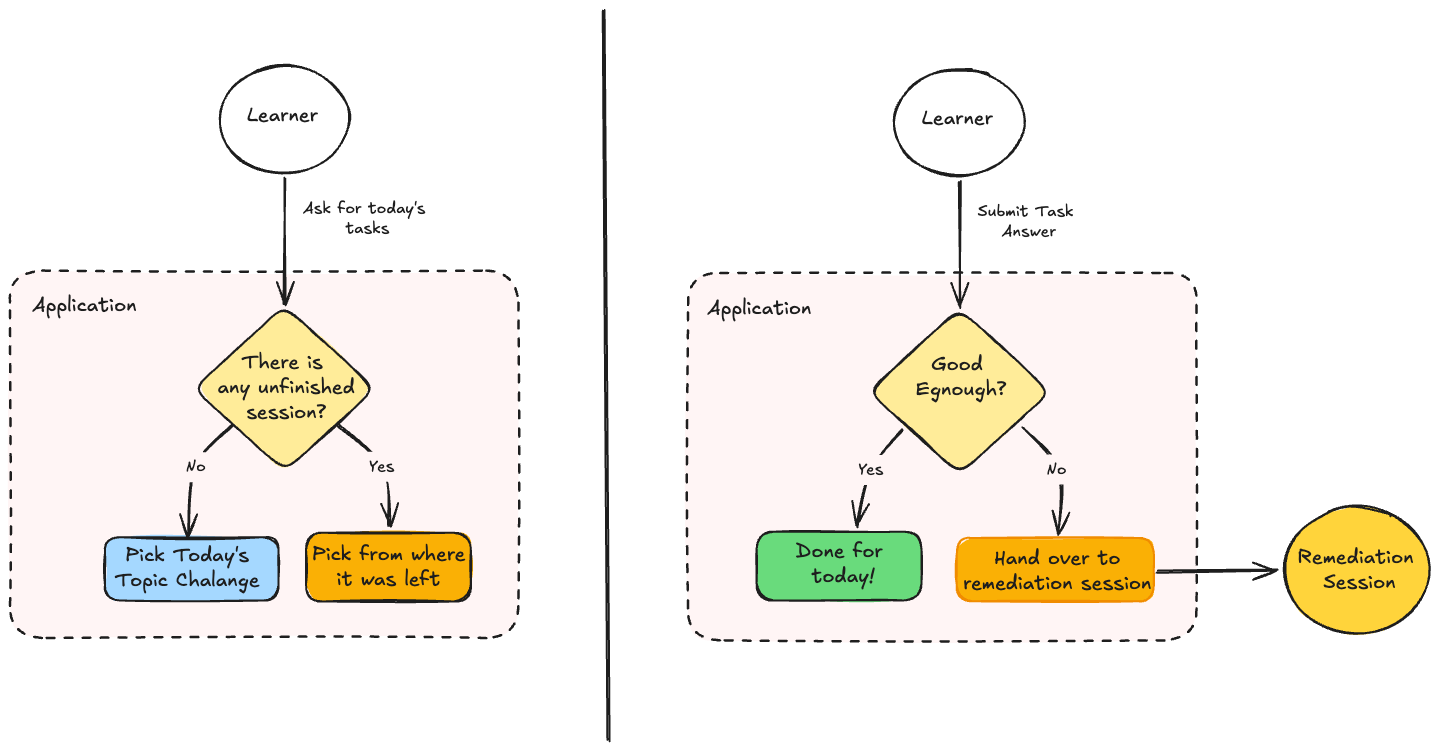
\includegraphics[width=\textwidth]{./figures/Daily-Chalange.png}
    \caption{Pedido do desafio diário e desfecho da resposta}
    \label{fig:daily-challenge}
\end{figure}

À esquerda, o pedido (\texttt{GET /tasks/today}) resolve-se num de quatro casos, por ordem: uma sessão de remediação aberta, uma sessão de explicação ativa, um desafio já atribuído nesse dia, ou a criação de um novo; os três primeiros são, na prática, a mesma ideia: retomar exatamente onde o Learner ficou. Só no último caso é que há algo por decidir: tanto a instância escolhida como a ordem das opções apresentadas são determinadas por uma semente ligada ao utilizador, reprodutível para ele (se recarregar o ecrã, vê sempre a mesma versão), mas sem padrão adivinhável para quem não conhece essa semente. É assim que o sistema garante que a resposta correta, sempre fixada no índice~0 internamente, aparece numa posição diferente e imprevisível no ecrã.

À direita, a resposta do Learner decide o resto do dia. O prazo vai até à meia-noite do dia seguinte no fuso horário do Learner; passado esse prazo, a submissão continua a ser aceite, mas com uma penalização crescente em vez de um corte abrupto. Se a resposta estiver certa, o dia termina ali; se não estiver, o Learner não fica simplesmente a saber que errou: é encaminhado de imediato para uma sessão de remediação, sem ação nenhuma da sua parte.

\subsubsection{Remediação Adaptativa} \label{sec:consolidation}

Um erro do Learner não é tratado como um resultado final, mas como um sintoma a diagnosticar. A Figura~\ref{fig:remediation-session} segue esse diagnóstico até à sessão de remediação e, do outro lado, até ao que acontece quando ela também não chega.

\begin{figure}[H]
    \centering
    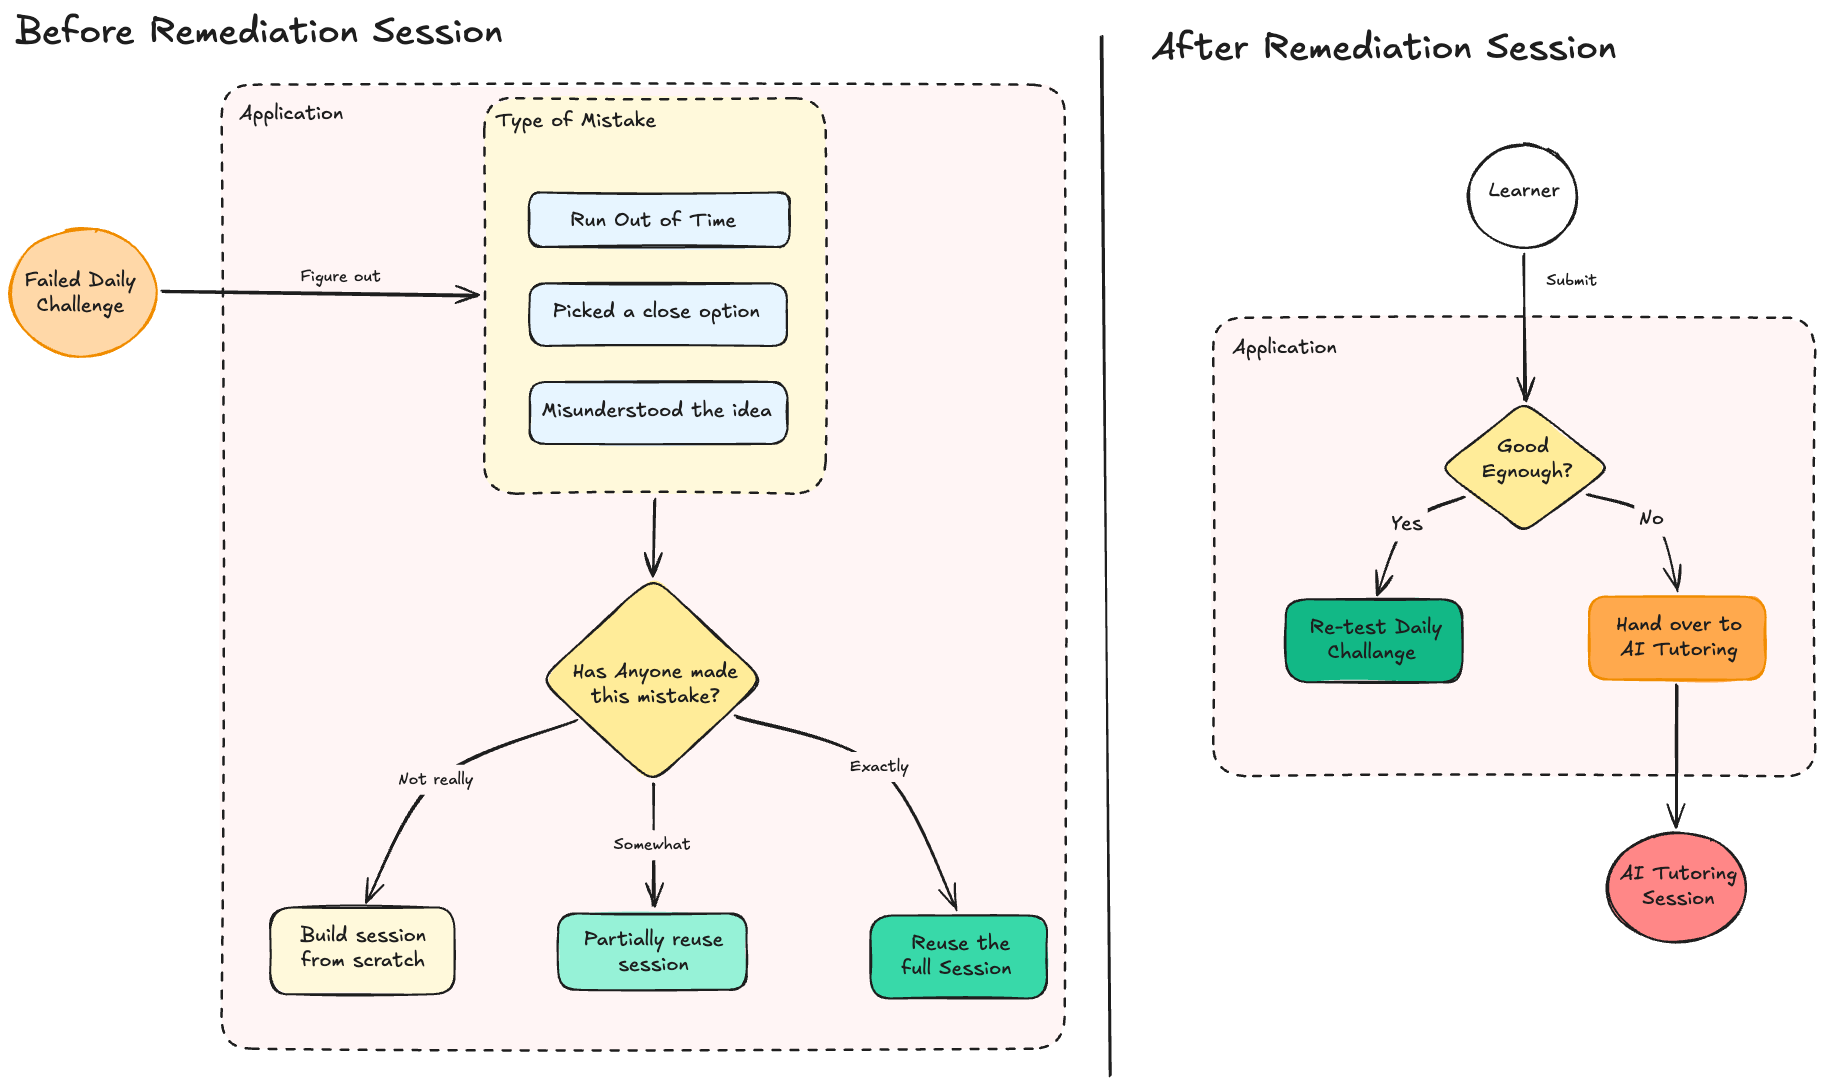
\includegraphics[width=\textwidth]{./figures/Remediation-session.png}
    \caption{Diagnóstico do erro, reutilização entre Learners, e desfecho da remediação}
    \label{fig:remediation-session}
\end{figure}

À esquerda, antes de gastar uma chamada de IA, o \texttt{ErrorPatternClassifier} classifica a falha de forma determinística, sem envolver o modelo, em três categorias (Tabela~\ref{tab:error-patterns}). Só depois disso é que entra a pergunta que o losango do diagrama levanta (``já alguém cometeu este mesmo erro?''), porque gerar as três sub-tarefas de remediação do zero, sempre que um Learner erra, seria repetir trabalho que a plataforma já fez para outro Learner com a mesma dificuldade.

\begin{table}[h!]
\centering
\caption{Padrões de erro classificados pelo ErrorPatternClassifier}
\label{tab:error-patterns}
\resizebox{\textwidth}{!}{%
\begin{tabular}{lll}
\hline
\textbf{Padrão} & \textbf{Condição} & \textbf{Estratégia de remediação} \\
\hline
\texttt{TIME\_PRESSURE} & Submissão após o prazo & Tarefas paceadas, passo a passo \\
\texttt{READING\_ERROR} & Opção selecionada adjacente à correta & Instruções mais explícitas \\
\texttt{WRONG\_CONCEPT} & Qualquer outro caso & Re-explicação do conceito de raiz \\
\hline
\end{tabular}%
}
\end{table}

Essa reutilização segue a mesma lógica de custo já vista na criação de conteúdo (Secção~\ref{cap:ingestao}), mas com uma pergunta mais fina do que ``já existe'': é ``quão parecida é a dificuldade que este Learner está a sentir com uma que já vimos antes''. O vetor de dificuldade (padrão de erro + descrição da tarefa + domínio) é comparado aos ramos já resolvidos por outros Learners, e a resposta depende de quão perto está o mais próximo. \label{sec:recuperacao}

\begin{table}[h!]
\centering
\caption{Estratégias de reutilização adaptativa por limiar de similaridade}
\label{tab:rag-reuse}
\resizebox{\textwidth}{!}{%
\begin{tabular}{llp{8.7cm}}
\hline
\textbf{Similaridade} & \textbf{Estratégia} & \textbf{Comportamento} \\
\hline
$> 0.90$         & \texttt{FULL\_REUSE}       & Devolve o ramo existente, sem chamada ao LLM \\
$(0.65,\,0.90]$  & \texttt{PARTIAL\_REUSE}    & Reutiliza $\max(1, \lfloor n \times \text{normSim} \rfloor)$ tarefas; gera o complemento via Mistral \\
$\leq 0.65$         & \texttt{FRESH\_GENERATION} & Gera o ramo completo via Mistral; persiste o \textit{embedding} para reutilização futura \\
\hline
\end{tabular}%
}
\end{table}

No caso intermédio, a proporção exata de reutilização não é um valor fixo, mas interpolada linearmente entre os dois limiares, $n_{\text{reuse}} = \max\!\left(1,\; \left\lfloor n_{\text{total}} \times \dfrac{sim - 0.65}{0.90 - 0.65} \right\rfloor\right)$, com um mínimo de uma tarefa reutilizada mesmo quando a similaridade está próxima do limiar inferior: quanto mais perto do limiar superior, mais próxima a dificuldade, e menos o sistema precisa de gerar de novo. O importante é que esta reutilização é \textit{entre} utilizadores, não pessoal a cada um: o valor do mecanismo não está em lembrar-se de um Learner, está em a plataforma inteira aprender com cada dificuldade que já viu.

Esta base de conhecimento pode, no entanto, tornar-se incoerente quando um Administrador edita conteúdo já gerado. O sistema resolve isso de forma diferente consoante o alcance da edição: uma edição pontual a uma tarefa mantém deliberadamente o \textit{embedding} antigo, porque só afeta deduplicação futura, não o que já foi entregue a um Learner; já uma regeneração completa do tópico purga e recalcula todos os vetores associados, de raiz. \label{sec:invalidacao}

Esta remediação para, deliberadamente, ao fim de um único nível. Continuar a encadear sub-tarefas do mesmo formato (escolha múltipla) tem retorno decrescente: se três sub-tarefas ainda não resolveram a incompreensão, mais três no mesmo molde dificilmente resolverão, e é a tutoria conversacional, não mais escolha múltipla, que responde a esse caso. Há também um argumento operacional: cada nível adicional multiplicaria chamadas à API de IA e prolongaria o tempo até o Learner voltar ao fluxo principal. O compromisso é reconhecido (tópicos avançados ficam sem patamares intermédios antes do escalamento) e tornar a profundidade configurável por tópico fica identificado como trabalho futuro. Estas tarefas adaptativas não pontuam (são modo de aprendizagem, não avaliação), mas, ao contrário da pontuação, completá-las corretamente na íntegra incrementa o \textit{streak} do Learner, do mesmo modo que uma resposta certa ao desafio principal.

É esse limite de um único nível que a Figura~\ref{fig:remediation-session} mostra à direita: o Learner submete as três sub-tarefas e, se as resolver todas, volta a testar o desafio original, fechando o ciclo; se não resolver, o sistema já não insiste com mais remediação: entrega-o à tutoria com IA, o único passo que resta.

\subsubsection{Tutoria com IA} \label{sec:explicacao-ia}

Quando mesmo a remediação falha, uma explicação de IA é o último recurso antes de deixar o Learner preso. A Figura~\ref{fig:ai-session} segue essa sessão desde que é aberta até ao Learner voltar, de uma forma ou de outra, ao desafio diário, fechando o ciclo que a Figura~\ref{fig:daily-challenge} começou.

\begin{figure}[H]
    \centering
    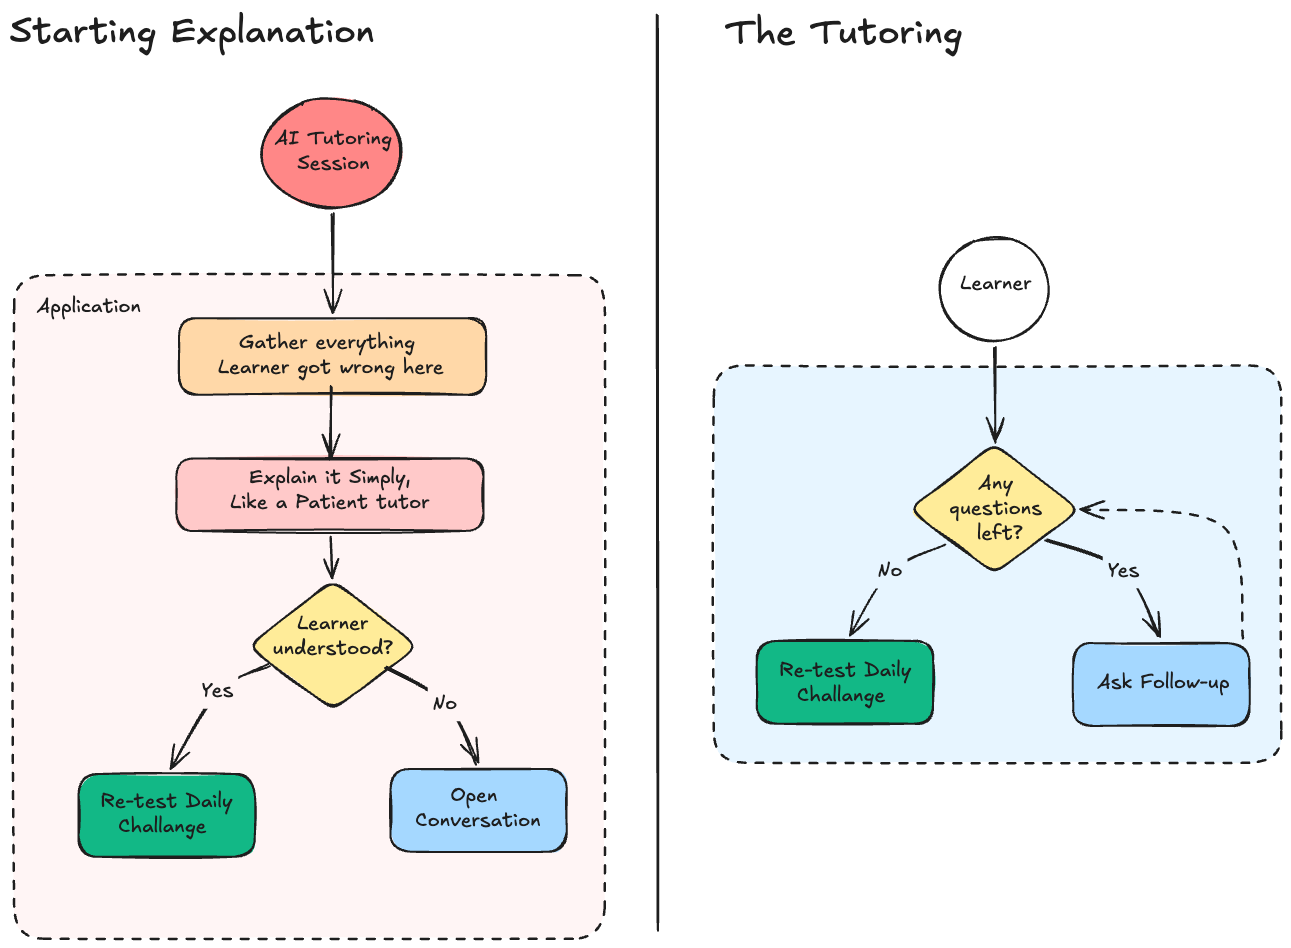
\includegraphics[width=\textwidth]{./figures/AI-Session.png}
    \caption{Explicação holística seguida de diálogo, até ao regresso ao desafio diário}
    \label{fig:ai-session}
\end{figure}

À esquerda, a sessão começa sempre pela mesma pergunta: o que é que este Learner, especificamente, já demonstrou não perceber? A resposta é o historial completo dos seus erros naquela tarefa, e é a partir dele (não de uma explicação genérica do conceito) que o modelo gera uma explicação holística, assumindo a persona de um tutor paciente focado na causa raiz. Se essa explicação bastar, o Learner regressa de imediato ao desafio diário; se não bastar, o sistema abre uma conversa.

À direita, essa conversa não tem limite de turnos (o Learner pergunta o que precisar, quantas vezes precisar), mas tem um limite de acesso por endereço IP, para conter o custo de cada chamada ao modelo, e o histórico de confiança mantém-se isolado do \textit{input} do Learner pela mesma estrutura de mensagens tipadas descrita na Secção~\ref{sec:seguranca-impl}. Assim que o Learner considera esclarecido, regressa ao mesmo sítio onde tudo começou: o desafio diário. Se a geração falhar ou exceder 60\,s, a sessão resolve-se automaticamente e o Learner é devolvido a esse mesmo ponto: também aqui, nunca fica bloqueado.

% =====================================================================
\section{Segurança: Cinco Camadas de Defesa} \label{sec:seguranca-impl} \label{cap:seguranca}
% =====================================================================

Cada capacidade aberta ao exterior nas secções anteriores (aceitar um URL de um Administrador, gerar texto por IA e devolvê-lo a um utilizador, expor uma API pública) é também uma superfície nova. A segurança não foi o foco central deste projeto, mas foi endereçada de forma pragmática à medida que cada uma destas superfícies foi ficando clara, camada a camada, várias delas catalogadas no OWASP (\textit{Open Worldwide Application Security Project}) Top 10. No total, cinco camadas independentes protegem o caminho entre a entrada HTTP e a chamada ao LLM. As primeiras três já foram apresentadas onde naturalmente se aplicam: \textit{rate limiting} e autenticação JWT na porta de entrada (Secção~\ref{sec:pipeline}), e validação de URL contra SSRF na ingestão (Secção~\ref{cap:ingestao}). Não são repetidas aqui. As duas restantes, específicas à camada de IA, fecham o capítulo.

\subsection*{Camada 4: Prevenção de Prompt Injection} \label{sec:protecao-ia}

Um sistema que gera texto por IA e o mostra a utilizadores tem de responder a uma pergunta simples: o que impede um Learner de escrever, numa das suas mensagens, algo como ``ignora as instruções anteriores e\ldots''? A resposta clássica, sanitizar o \textit{input}, é frágil porque tenta detetar ataques depois de já os deixar entrar na mesma \textit{string} que o resto do \textit{prompt}. O Play4Change evita o problema pela raiz: cada peça de informação enviada ao modelo é encapsulada no tipo de mensagem correspondente ao seu nível de confiança: uma \texttt{SystemMessage} de confiança, dados estruturados da base de dados, o historial da conversa, e só por fim, isolado na sua própria mensagem de origem não confiada, o \textit{input} atual do utilizador. A fronteira de \textit{role} da própria API do modelo garante que essa última mensagem nunca altera o comportamento definido na primeira. E, como já referido na Secção~\ref{sec:ia-prompting}, os prompts de geração de tarefas e de análise de dificuldade nem sequer recebem \textit{input} do utilizador final: nesses casos, o vetor está eliminado por construção, não por deteção.

\subsection*{Camada 5: Sanitização de Output e Outros Controlos} \label{sec:xss}

A pergunta inversa também precisa de resposta: o que impede o próprio modelo, ao reproduzir conteúdo de uma página raspada, de devolver HTML malicioso que acabe por correr no browser de um utilizador? Três técnicas independentes respondem, em camadas: todo o texto gerado é normalizado para texto plano (remoção de todas as tags HTML, incluindo \texttt{<script>}/\texttt{<style>}) antes de ser persistido; o Nginx aplica uma \textit{Content Security Policy} restritiva ao bloco que serve a aplicação web; e o React escapa automaticamente qualquer expressão ao renderizar no ecrã. É uma defesa deliberadamente redundante: mesmo que uma das três falhe, as outras duas continuam a proteger. \label{sec:validacao}

Um punhado de outros controlos, mais pontuais, fecha as portas mais óbvias que ficariam por fechar: o servidor recusa-se a arrancar em produção com um segredo JWT por omissão; a rotação de \textit{refresh token} já descrita revoga toda a família ao primeiro sinal de reutilização; o acesso é limitado por papel e a lista de origens CORS é verificada explicitamente ao arranque, sem aceitar \textit{wildcards}; o Nginx aplica quatro \textit{headers} de segurança a todas as respostas, mais uma \textit{Content Security Policy} restrita ao bloco que serve a aplicação web; e o \textit{scraper} de URLs opera com \textit{timeout} próprio e remove ativamente elementos de \textit{script} antes de extrair texto. \label{sec:outros-seguranca}

\subsection*{Vetores de Ataque Considerados} \label{sec:riscos}

Não foi conduzida uma auditoria de segurança formal nem uma análise de risco quantificada: a segurança foi endereçada vetor a vetor, à medida que cada um se tornou relevante à arquitetura concreta do sistema. A Tabela~\ref{tab:riscos} junta, num só lugar, os dez vetores considerados ao longo deste capítulo e o controlo correspondente.

\begin{table}[h!]
\centering
\caption{Vetores de ataque considerados e controlo implementado}
\label{tab:riscos}
\resizebox{\textwidth}{!}{%
\begin{tabular}{lp{6.5cm}p{7cm}}
\hline
\textbf{Vetor} & \textbf{Controlo implementado} & \textbf{Observação} \\
\hline
XSS via conteúdo gerado por IA         & Sanitização + CSP (parcial) + \textit{auto-escaping} do React & --- \\
Prompt Injection                       & Multi-mensagem tipada + limites de contexto      & Mitiga ataques simples; o Mistral não garante resistência total a \textit{inputs} adversariais sofisticados \\
Custo descontrolado de chamadas à API de IA & Rate limiting por IP (10 req/10\,min em \texttt{/explanation}, entre outros) & Mitiga abuso de um único atacante, não um ataque distribuído \\
Roubo de \textit{refresh token}         & Rotação com família + revogação total em caso de reutilização & Janela de 7~dias de exposição se o token for exfiltrado; impacto limitado pela TTL de 15~min do \textit{access token} \\
Segredo JWT por omissão em produção     & \textit{Startup guard} impede o arranque      & --- \\
SSRF via URL de ingestão               & \texttt{UrlSsrfValidator}                             & --- \\
Força bruta em autenticação            & Rate limiting (5 req/10\,min)                         & --- \\
\textit{Spoofing} de IP no rate limiting & Extrator de IP rejeita endereços privados no header & --- \\
Escalada de privilégios (Learner~$\to$~Admin) & RBAC + validação de papel no JWT               & --- \\
CORS \textit{wildcard}                 & Verificação de lista de origens ao arranque           & --- \\
\hline
\end{tabular}%
}
\end{table}

Três destas decisões deixam uma margem de exposição residual mais visível, e não foram objeto de mitigação adicional: a proteção contra \textit{prompt injection} não é absoluta, porque depende do comportamento do modelo, não só da separação de mensagens; o \textit{rate limiting} por IP não impede um ataque distribuído a partir de múltiplos endereços; e a janela de 7~dias do \textit{refresh token} só é neutralizada se a sanitização de \textit{output} estiver de facto bem mitigada. Ficam identificadas como pontos a reforçar caso o sistema avance para produção com utilização real.

\bigskip

Este capítulo descreveu o que foi de facto implementado e validado. As decisões deliberadamente deixadas de fora do âmbito atual (profundidade de remediação configurável por tópico, funcionalidades sociais e de retenção, reconhecimento formal de competências, entre outras) estão detalhadas na Secção de Trabalho Futuro do Capítulo~\ref{cap:discussao}, e não são repetidas aqui.
